\documentclass[11pt,a4paper]{article}

% --- Encoding and language ---
\usepackage[utf8]{inputenc}
\usepackage[T1]{fontenc}
\usepackage[english]{babel}

% --- Layout ---
\usepackage[margin=2.4cm]{geometry}
\usepackage{setspace}
\onehalfspacing

% --- Math, figures, tables ---
\usepackage{amsmath,amssymb}
\usepackage{graphicx}
\graphicspath{{figures/}}
\usepackage{booktabs}
\usepackage{float}
\usepackage{caption}
\usepackage{subcaption}
\usepackage{xcolor}

% --- Links ---
\usepackage[colorlinks=true,linkcolor=blue!60!black,urlcolor=blue!60!black,citecolor=blue!60!black]{hyperref}

\title{\textbf{Multi-drone patrolling:\\ persistent coverage with heuristic search}}
\author{Emile Descroix - Anaël Ernadote}
\date{Modeling and Problem Solving - M2\\ Université Paris-Dauphine - PSL}

\begin{document}

\maketitle

\begin{abstract}
\noindent
How can $N$ drones be coordinated to monitor an area continuously, so that no
place stays ``blind'' for too long? The report follows this approach: we
implement an algorithm, measure its performance, identify its limits, then move
on to another algorithm from the course that may fix them. We thus go through two
families of heuristic search methods: first \emph{reactive / MAPF} strategies
(Dijkstra, space-time A\textsuperscript{*}, ALT, Conflict-Based Search, Partial
Move A\textsuperscript{*}), then a \emph{global optimization} of patrol cycles
(hill climbing, genetic algorithm, NRPA). The main result is that bounding the
idleness with optimized cycles divides the worst idleness by a factor of
$\approx 2.5$, whereas refining the reactive coordination alone does not.
\end{abstract}

\newpage
\tableofcontents
\newpage

% ======================================================================
\section{Introduction}
% ======================================================================

Monitoring an area with a fleet of drones is not a classic \emph{coverage}
problem: visiting each cell once is not enough, each cell must be
\emph{revisited regularly}. This variant is called \emph{multi-agent
patrolling}. It arises whenever a phenomenon evolves over time (emerging fires,
intrusions, environmental measurements) and information gets older as long as it
is not observed.

The problem combines several building blocks from the heuristic search course:
shortest paths (Dijkstra, A\textsuperscript{*}), \emph{Multi-Agent Path Finding}
(MAPF) and its solvers (prioritized planning, Conflict-Based Search, Partial Move
A\textsuperscript{*}), and combinatorial optimization with metaheuristics (local
search, genetic algorithm, NRPA).

The report is deliberately \textbf{sequential}: each section implements an
algorithm, evaluates its performance on the same reference instance, then
motivates the next algorithm by the limit observed. All figures are produced by
the project code (\texttt{generate\_figures.py}) to ensure reproducibility.

% ======================================================================
\section{Modeling}
% ======================================================================

\paragraph{Environment.} The area is a $W \times H$ grid with 4-connectivity.
Some cells are \emph{obstacles} (no-fly zones that cannot be crossed). A drone
moves by one cell per time step (North, East, South, West, or wait), exactly
under the MAPF assumptions of the course: \emph{``each agent can move N, E, S or
W into any adjacent unblocked cell''}.

\paragraph{Sensor.} A drone on cell $c$ observes every free cell within a
Euclidean disk of radius $R$ around $c$. The view is not occluded: drones fly
over obstacles.

\paragraph{Idleness.} Each free cell $c$ has an \emph{idleness} $\tau(c,t)$: the
number of steps since it was last observed. At each time step, every cell ages
by $1$, and observed cells go back to $0$:
\[
  \tau(c, t{+}1) =
  \begin{cases}
    0 & \text{if } c \text{ is observed at } t{+}1,\\[2pt]
    \tau(c,t) + 1 & \text{otherwise.}
  \end{cases}
\]

\paragraph{Objective.} We want to minimize the \textbf{maximum idleness} in
steady state, $\max_c \tau(c,t)$ (the worst blind area), and secondarily the
mean idleness. Figure~\ref{fig:coverage} illustrates the stakes: a greedy
strategy can leave a large area unmonitored (light on the heat map), whereas a
cycle-based strategy keeps a uniform coverage.

\begin{figure}[H]
  \centering
  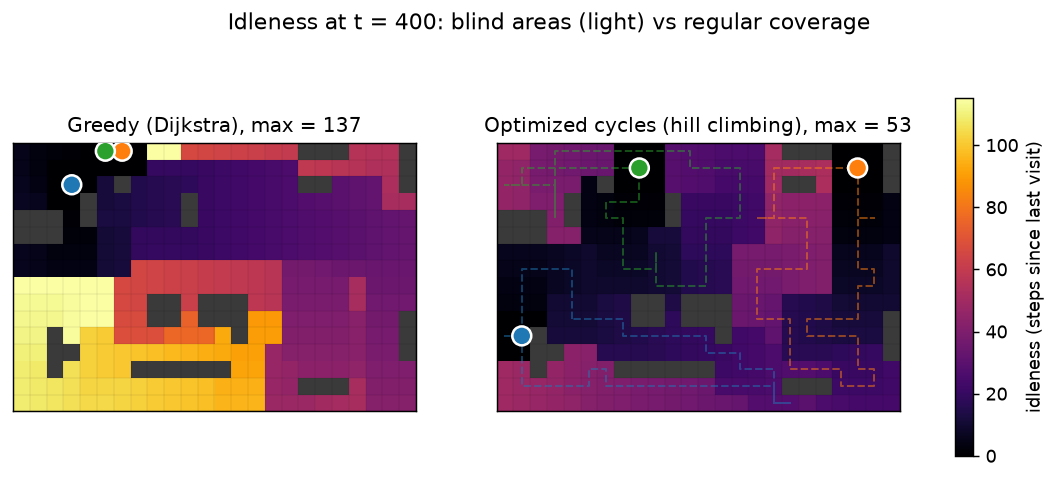
\includegraphics[width=\linewidth]{fig1_coverage.png}
  \caption{Idleness map at $t=400$ ($24\times16$ grid, 3 drones). Left, the
  greedy baseline: the two top drones have clustered together and a whole region
  (light yellow) has stayed blind for $\approx 137$ steps. Right, the optimized
  cycles (dashed lines): coverage is regular and the maximum idleness drops to
  $53$.}
  \label{fig:coverage}
\end{figure}

\paragraph{Reference instance.} Unless stated otherwise, all evaluations use
the same instance: $24\times16$ grid, $12\,\%$ obstacles, radius $R=1.5$, $3$
drones, random seed $42$, and $400$ simulation steps, of which only the second
half is averaged (steady state).

% ======================================================================
\section{Approach: two families of algorithms}
% ======================================================================

We compare two paradigms, both taken from the course.

\begin{description}
  \item[Family A: reactive / MAPF.] At each time step, each drone picks a
  ``cold'' target and a solver coordinates the moves without collision. We
  progressively refine the \emph{pathfinding} (Dijkstra, then
  A\textsuperscript{*}, then ALT) and the \emph{coordination} (priorities, then
  CBS, then PMA\textsuperscript{*}).
  \item[Family B: global optimization.] We precompute patrol \emph{cycles} that
  \emph{bound} the idleness, then optimize these cycles with metaheuristics (hill
  climbing, genetic algorithm, NRPA).
\end{description}

The common thread of the following sections: family~A improves
\emph{safety} and smoothness, but runs into a variable and rather greedy
coverage; family~B changes paradigm and brings the idleness down.

% ======================================================================
\section{Family A: reactive strategies and MAPF}
% ======================================================================

All these strategies share the same \emph{target choice}. A drone at position
$p$ targets the cell $c$ that maximizes a score combining urgency and proximity:
\begin{equation}
  \operatorname{score}(c) = \tau(c,t) - \alpha \, d(p, c),
  \label{eq:score}
\end{equation}
where $d(p,c)$ is the shortest-path distance and $\alpha$ a weight. Only the way
paths are \emph{planned} and \emph{coordinated} changes.

% ----------------------------------------------------------------------
\subsection{Greedy baseline (Dijkstra)}
% ----------------------------------------------------------------------

\paragraph{Implementation.} The distance $d$ in equation~\eqref{eq:score} is
computed with \textbf{Dijkstra}, then the drone follows the shortest path to its
target. There is no coordination: we only prevent two drones from picking the
same target, and move conflicts are resolved naively by index priority (the
lowest index moves, the other waits).

\paragraph{Evaluation.} It is a fair baseline: maximum idleness $\approx 136$,
mean $\approx 52$ (table~\ref{tab:results}). But the policy is optimal at time
$t$ and not at $t+1$: two drones can converge to the same region and abandon
another one (figure~\ref{fig:coverage}, left). Moreover, resolving conflicts by
simple priority can make two drones overlap in edge cases.

\paragraph{Limit $\Rightarrow$ next step.} We need a coordination that
\emph{guarantees} the absence of collisions: we move on to space-time planning.

% ----------------------------------------------------------------------
\subsection{Space-time A\texorpdfstring{\textsuperscript{*}}{*}}
% ----------------------------------------------------------------------

\paragraph{Implementation.} We plan in the state space $(\text{cell}, t)$.
A\textsuperscript{*} expands the leaf with the smallest $f = g + h$, using the
Manhattan heuristic $h(c,g)=|x_c-x_g|+|y_c-y_g|$, which is admissible because it
ignores obstacles and other drones. The paths of higher-priority drones are
written into a \textbf{reservation table} that forbids vertex collisions
($(c,t)$ occupied) and edge collisions (head-on swaps). The table is never built
explicitly: reserved states are simply not \emph{generated}. This is
\emph{prioritized planning} / \emph{Cooperative Pathfinding} by Silver~(2005).

\paragraph{Evaluation.} Safety is achieved (zero collisions), but the idleness
does not improve; it even gets worse ($\approx 161$, table~\ref{tab:results})
because the waits imposed by priorities slow down the coverage. Above all, the
priority order is \emph{fixed} (drone index): the method is \textbf{neither
complete nor optimal}.

\paragraph{Limits $\Rightarrow$ two directions.} (i) The Manhattan heuristic is
poorly informed in corridors: we improve it with ALT (§\ref{sec:alt}). (ii)
Priority-based coordination is fragile: we replace it with CBS (§\ref{sec:cbs})
then PMA\textsuperscript{*} (§\ref{sec:pma}).

% ----------------------------------------------------------------------
\subsection{ALT heuristic}
\label{sec:alt}
% ----------------------------------------------------------------------

\paragraph{Implementation.} \textbf{ALT} (A\textsuperscript{*}, Landmarks,
Triangle inequality) precomputes, with a Dijkstra from a few \emph{landmarks}
$L$, the true distances $d(L,\cdot)$. The triangle inequality then gives an
admissible lower bound that is tighter than Manhattan:
\begin{equation}
  h_{\mathrm{ALT}}(c,g) = \max_{L} \bigl| d(L,c) - d(L,g) \bigr| \;\le\; d(c,g).
  \label{eq:alt}
\end{equation}
Landmarks are chosen ``farthest-first'' (as far apart as possible). Unlike
Manhattan, ALT ``sees'' the obstacles.

\paragraph{Evaluation.} ALT does not change the patrol quality (same optimal
paths): it is a \emph{speed-up}. On a corridor grid ($40\times28$, $30\,\%$
obstacles), A\textsuperscript{*} expands $\approx 1.4\times$ fewer leaves
(figure~\ref{fig:alt}), while optimality is preserved. The gain grows with the
obstacle density.

\begin{figure}[H]
  \centering
  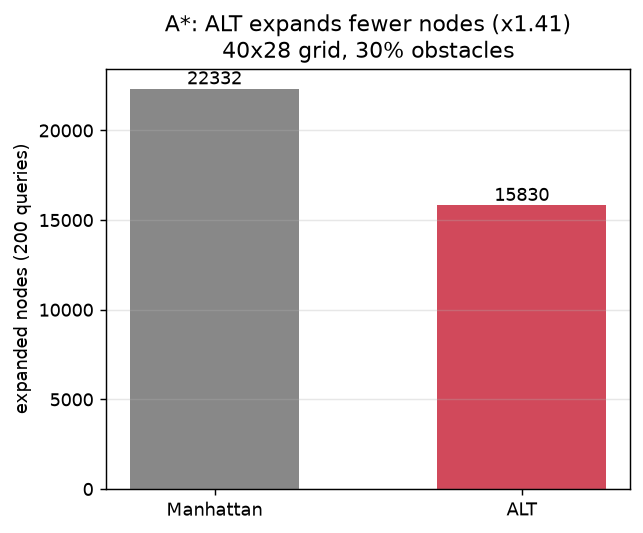
\includegraphics[width=0.52\linewidth]{fig5_alt.png}
  \caption{ALT versus Manhattan: total number of leaves expanded by
  A\textsuperscript{*} over $200$ shortest-path queries. The paths found are
  identical; ALT simply explores fewer nodes.}
  \label{fig:alt}
\end{figure}

% ----------------------------------------------------------------------
\subsection{Conflict-Based Search (CBS)}
\label{sec:cbs}
% ----------------------------------------------------------------------

\paragraph{Implementation.} \textbf{CBS} fixes the weakness of prioritized
planning. It works on two levels:
\begin{itemize}
  \item \emph{Low level}: for a given drone, a space-time A\textsuperscript{*}
  finds the shortest path under a set of \emph{constraints} (vertex or edge
  bans at given times).
  \item \emph{High level}: a binary tree. Each drone is first planned
  independently; we look for the first conflict; we create two children, each
  forbidding \emph{one} of the two conflicting drones from being there at that
  time, and we replan only that drone. The node with the lowest cost (sum of
  lengths) is always expanded first.
\end{itemize}
Unlike space-time A\textsuperscript{*}, CBS fixes no priority order: it is
\textbf{complete and optimal}.

\paragraph{Evaluation.} CBS does produce collision-free trajectories. It
\emph{smooths} the coverage: it is the reactive strategy with the lowest
\emph{mean} idleness ($\approx 49$, table~\ref{tab:results}). However, the
\emph{maximum} idleness stays at $\approx 138$, in the same range as the
baseline: better coordination does not fix the intrinsically greedy nature of
equation~\eqref{eq:score}.

% ----------------------------------------------------------------------
\subsection{Partial Move A\texorpdfstring{\textsuperscript{*}}{*}}
\label{sec:pma}
% ----------------------------------------------------------------------

\paragraph{Implementation.} We can search directly in the \emph{joint} space of
the $N$ drones (their simultaneous positions). This is optimal but explodes: a
full move is a combination of one action per drone, i.e. up to $5^N$ successors
per node. \textbf{Partial Move A\textsuperscript{*}} keeps the same space but
\emph{stops the search after each partial action}: a node fixes the cells of
drones $0..k{-}1$, and only one drone is added at a time, immediately pruning
collisions with the drones already fixed. The branching factor drops from $5^N$
to~$5$.

\paragraph{Evaluation (as a solver).} On position-swap instances, the gain grows
strongly with the number of drones: PMA\textsuperscript{*} generates up to
$\approx 18\times$ fewer successors than joint A\textsuperscript{*} for $4$
drones (figure~\ref{fig:pma}), for the same optimal path.

\begin{figure}[H]
  \centering
  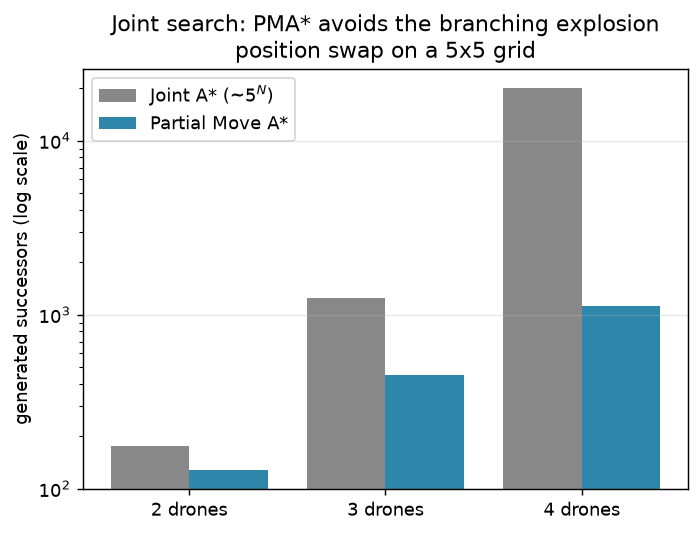
\includegraphics[width=0.62\linewidth]{fig6_pma.png}
  \caption{Joint search: generated successors (log scale). Joint
  A\textsuperscript{*} suffers from a $5^N$ branching factor;
  PMA\textsuperscript{*} avoids it with partial expansion. The gap widens as the
  number of drones grows.}
  \label{fig:pma}
\end{figure}

\paragraph{Evaluation (in patrolling).} Once integrated into the patrol,
PMA\textsuperscript{*} is nevertheless the \emph{worst} ($\approx 191$,
table~\ref{tab:results}). The reason is instructive: its joint plan is optimal in
\emph{makespan}, so drones that reach their target early \emph{wait} for the
others before everyone is replanned. \emph{This forced waiting degrades the
coverage.} This is a central lesson: \textbf{MAPF optimality is not the patrol
objective}. The real value of CBS and PMA\textsuperscript{*} is as
\emph{solvers}, not as coverage policies.

% ----------------------------------------------------------------------
\subsection{Summary of family A}
% ----------------------------------------------------------------------

Figure~\ref{fig:comparison} overlays the idleness over time for all strategies.
The reactive curves (greedy, A\textsuperscript{*}, CBS, PMA\textsuperscript{*})
\emph{drift}: the worst area keeps getting darker, because the target choice
remains local. None of these methods \emph{guarantees} that a given cell will be
revisited. This is precisely what family~B provides.

\begin{figure}[H]
  \centering
  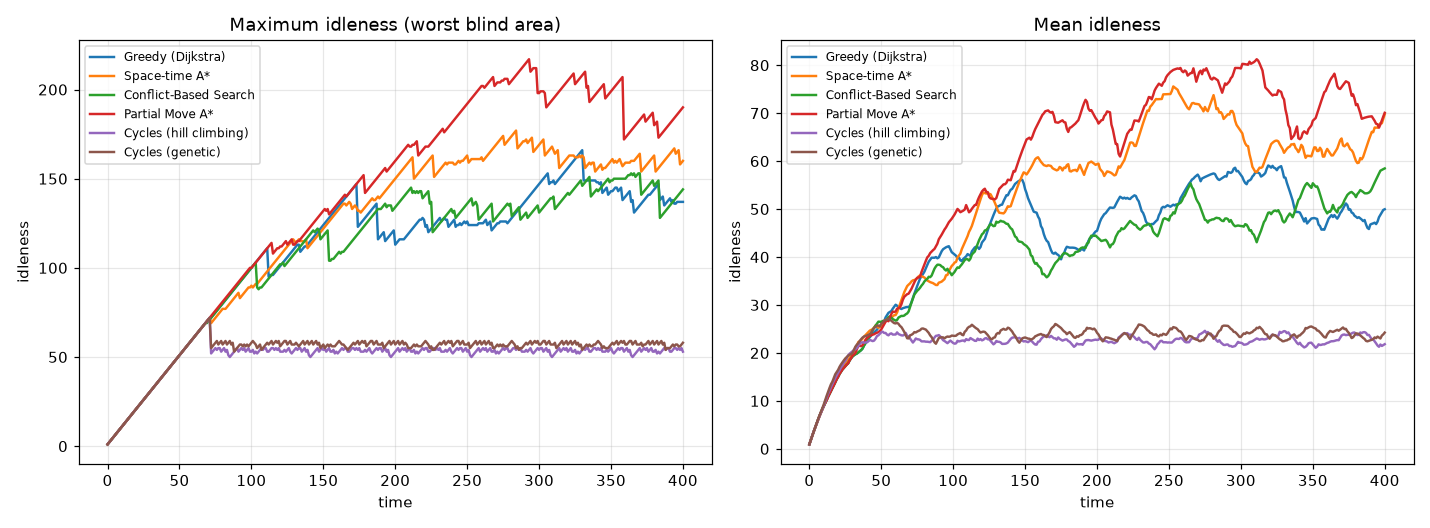
\includegraphics[width=\linewidth]{fig2_comparison.png}
  \caption{Maximum (left) and mean (right) idleness over time. Reactive
  strategies (family~A) drift upwards; cycle-based strategies (family~B,
  purple/brown) settle low and flat.}
  \label{fig:comparison}
\end{figure}

% ======================================================================
\section{Family B: global optimization with cycles}
% ======================================================================

% ----------------------------------------------------------------------
\subsection{Reduction to a multi-TSP}
% ----------------------------------------------------------------------

The key idea: if a drone follows a closed \emph{cycle} of $L$ steps, each cell of
its area is revisited at least once every $L$ steps. The maximum idleness is then
\textbf{bounded} by the length of the longest cycle, which reactive strategies
never guarantee. The cycles are built in three steps:

\begin{enumerate}
  \item \textbf{Coverage}: a greedy \emph{set cover} heuristic picks a small set
  of \emph{waypoints} such that every free cell is seen from at least one of
  them.
  \item \textbf{Distances}: one Dijkstra per waypoint gives the matrix $D$ of
  shortest paths between waypoints.
  \item \textbf{Tours}: the waypoints are partitioned among the $N$ drones and
  each part is ordered into a cycle, which is a \emph{multi-TSP}. The cost to
  minimize directly approximates the patrol objective:
  \begin{equation}
    \text{cost}(\text{routes}) = \max_d L_d + 0.1\cdot\overline{L},
    \label{eq:cost}
  \end{equation}
  where $L_d$ is the cycle length of drone $d$ and $\overline{L}$ the mean (the
  mean term breaks ties between solutions with the same longest cycle).
\end{enumerate}

This multi-TSP is optimized with three metaheuristics, compared \textbf{with the
same evaluation budget}.

% ----------------------------------------------------------------------
\subsection{Hill climbing}
% ----------------------------------------------------------------------

\paragraph{Implementation.} Local search on the routes, with three classic tour
operators: \emph{2-opt} (reverse a segment), \emph{relocate} (move a waypoint to
the best insertion point of another cycle), \emph{swap} (exchange two waypoints
between cycles). Sideways moves (plateaus) are accepted and the search restarts
randomly on stagnation, keeping the best solution found. Moves target the
longest cycle first, since it sets the cost~\eqref{eq:cost}.

\paragraph{Evaluation.} This is the big leap: maximum idleness $\approx 54$,
i.e. divided by $\approx 2.5$ compared with family~A (table~\ref{tab:results}).
Figure~\ref{fig:cycles} shows the cycles obtained: three compact and disjoint
loops, each assigned to one drone.

\begin{figure}[H]
  \centering
  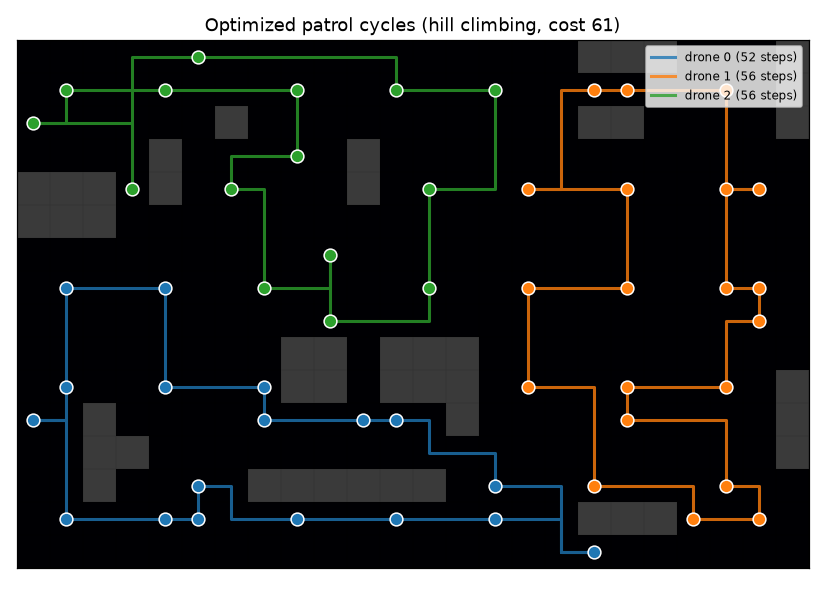
\includegraphics[width=0.72\linewidth]{fig4_cycles.png}
  \caption{Patrol cycles optimized by hill climbing. Each drone loops over a
  compact region; the length of the longest cycle bounds the maximum idleness.}
  \label{fig:cycles}
\end{figure}

% ----------------------------------------------------------------------
\subsection{Genetic algorithm}
% ----------------------------------------------------------------------

\paragraph{Implementation.} Multi-TSP representation:
\[
  \text{chromosome} = (\text{permutation of the waypoints},\ N{-}1\text{ cuts}).
\]
OX crossover (\emph{Order Crossover}), mutations (swap, segment reversal, cut
shift), tournament selection and elitism.

\paragraph{Evaluation.} With the same budget, the genetic algorithm is slightly
behind hill climbing ($\approx 57$ versus $\approx 54$). On a TSP-like
landscape, 2-opt local search exploits the neighborhood better than a GA without
built-in local search.

% ----------------------------------------------------------------------
\subsection{NRPA}
% ----------------------------------------------------------------------

\paragraph{Implementation.} \textbf{NRPA} (Nested Rollout Policy Adaptation;
Dang \emph{et al.}~2023) explores neither a neighborhood nor a population: it
\emph{learns a construction policy}. We use the \emph{route-first, split-second}
formulation, standard and efficient for the multi-TSP:
\begin{enumerate}
  \item NRPA learns a single large tour through all the waypoints: a classic
  TSP, a setting where NRPA excels. A ``move'' picks the next waypoint, encoded
  by the edge (last, next), with a probability given by the policy.
  \item This tour is split into $N$ contiguous segments (one per drone) by
  dynamic programming that minimizes the longest cycle.
\end{enumerate}
The \texttt{adapt} function reinforces the edges of the best tour; the recursion
nests several levels.

\paragraph{Evaluation.} With the same budget ($6000$ evaluations), NRPA converges
more slowly than hill climbing (cost $\approx 118$ versus $61$), because local
search dominates on a TSP of this size. Its correctness is confirmed by the
convergence with a growing budget (cost $\approx 88$ at $30\,000$ evaluations):
NRPA catches up with large budgets, where its world records on harder
combinatorial problems lie. Figure~\ref{fig:convergence} overlays the three
convergence curves.

\begin{figure}[H]
  \centering
  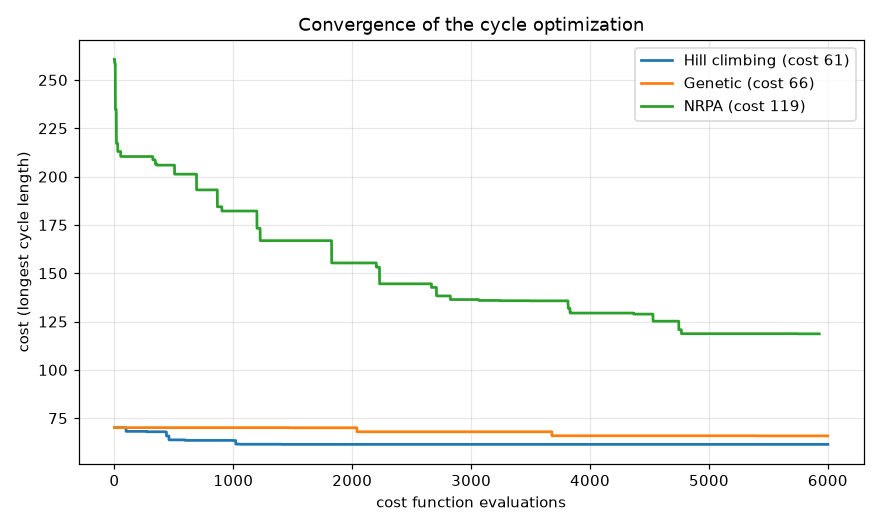
\includegraphics[width=0.7\linewidth]{fig3_convergence.png}
  \caption{Convergence of the three metaheuristics on the multi-TSP, with the
  same evaluation budget. Hill climbing goes down the fastest; NRPA converges
  more slowly at this budget.}
  \label{fig:convergence}
\end{figure}

% ======================================================================
\section{Consolidated results and discussion}
% ======================================================================

\begin{table}[H]
  \centering
  \caption{Steady-state idleness ($24\times16$ grid, $12\,\%$ obstacles, $3$
  drones, seed $42$, $400$ steps). Lower is better.}
  \label{tab:results}
  \begin{tabular}{llrr}
    \toprule
    Family & Strategy & Max idleness & Mean idleness \\
    \midrule
    A: reactive & Greedy (Dijkstra)                  & 135.8 & 52.1 \\
    A: reactive & Space-time A\textsuperscript{*}   & 161.4 & 65.3 \\
    A: reactive & Conflict-Based Search              & 138.4 & 49.2 \\
    A: reactive & Partial Move A\textsuperscript{*} & 190.7 & 73.3 \\
    \textbf{B: cycles} & \textbf{Cycles (hill climbing)} & \textbf{53.7} & \textbf{22.7} \\
    B: cycles & Cycles (genetic)                     & 57.2 & 23.9 \\
    \bottomrule
  \end{tabular}
\end{table}

Three lessons emerge.

\paragraph{1. Global optimization changes the order of magnitude.} Moving from
a reactive policy to optimized cycles divides the worst idleness by
$\approx 2.5$. This is the direct consequence of the \emph{bound} guaranteed by
the cycles: the worst case is \emph{under control}, whereas reactive strategies
offer no revisit guarantee (figure~\ref{fig:comparison}).

\paragraph{2. Within the reactive family, coordination matters little for the
maximum idleness.} CBS and the greedy baseline are neck and neck on the
\emph{max} ($\approx 138$ versus $136$); CBS only improves the \emph{mean}.
Improving the MAPF solver does not fix the underlying flaw, which justifies the
change of paradigm.

\paragraph{3. MAPF optimality $\ne$ good patrolling.}
PMA\textsuperscript{*}, although an excellent joint search \emph{solver}
(figure~\ref{fig:pma}), is the \emph{worst} at patrolling: its makespan
synchronization makes the drones wait. The right criterion is not the makespan
of an isolated move, but the idleness \emph{integrated over time}.

\paragraph{Algorithmic cost.} Reactive strategies replan at every step but remain
cheap (small grid); CBS and PMA\textsuperscript{*} make coordination heavier. On
the optimization side, hill climbing and the genetic algorithm converge in a
fraction of a second for $6000$ evaluations; NRPA is more expensive (a few
seconds) because of the dynamic programming split repeated at each
\emph{rollout}.

% ======================================================================
\section{Conclusion}
% ======================================================================

Following an incremental approach (implement, measure, fix), we went through a
large part of the heuristic search algorithms of the course, applied to the same
concrete problem. \textbf{The right algorithm depends on the right criterion}:
optimal MAPF solvers (CBS, PMA\textsuperscript{*}) shine at collision-free motion
but do not optimize persistent coverage, whereas the multi-TSP reduction directly
aligns the optimized cost with the maximum idleness and brings it down by a
factor of $2.5$.

\paragraph{Future work.} Running the family~B cycles with CBS coordination would
guarantee the absence of collisions \emph{without} losing the idleness bound; a
memetic GA or NRPA with a larger budget would tighten the optimization; finally,
idleness weighted by priority areas, heterogeneous drones or failures would bring
the model closer to a real deployment.

\end{document}
